\documentclass[11pt]{article}
\usepackage{mathblatt}
% gesetzt von werkzeuge/setzer.py (Sorte selbst) aus dem Lernweg FUR
% und den Bankzeilen; Muster bau/proben/2026-10-09/hypotenuse-muster.
\usepackage{enumitem}
\usepackage{adjustbox,varwidth}
\newgeometry{a4paper,margin=18mm,top=15mm,bottom=20mm,footskip=9mm}
\pagestyle{fancy}\fancyhf{}\renewcommand{\headrulewidth}{0pt}
\fancyfoot[L]{\footnotesize\color{mbgrau}FUR \textperiodcentered{} Zahlen vergleichen – auch negativ, mit Bruch, Prozent, Quadrat und Wurzel}
\fancyfoot[R]{\footnotesize\color{mbgrau}\thepage}
\setlength{\parskip}{3pt}
\renewcommand{\kreuz}[1]{\mbox{$\square$\ #1}\quad}
\providecommand{\kk}[1]{$\square$\,#1\hspace{0.9em}}
\providecommand{\linie}[1]{\,{\color{black!45}\rule[-1pt]{#1}{0.4pt}}\,}
\providecommand{\grau}[1]{{\color{mbgrau}#1}}
\newcommand{\kreuzl}[1]{\par\hangindent1.4em\hangafter1\noindent$\square$\ #1}
\newcommand{\aufg}[3]{\par\noindent\makebox[0pt][r]{#3}\begin{minipage}[t]{\linewidth}#1\end{minipage}\par}
\newcommand{\aufgg}[4]{\par\noindent\makebox[0pt][r]{#4}\begin{minipage}[t]{0.6\linewidth}\vspace{0pt}#1\end{minipage}\hfill
  \begin{minipage}[t]{0.37\linewidth}\vspace{0pt}\centering #2\end{minipage}\par}
\newcommand{\nr}[1]{\makebox[7mm][l]{\textbf{#1}}}
\newcommand{\lsg}[3]{\par\noindent\begin{minipage}[t]{9mm}\textbf{#1}\end{minipage}%
  \begin{minipage}[t]{52mm}\raggedright\bfseries\boldmath #2\end{minipage}\hspace{3mm}%
  \begin{minipage}[t]{\dimexpr\linewidth-64mm\relax}\raggedright\small #3\end{minipage}\par\vspace{4pt}}
\newlength{\kr}
\makeatletter
\newcommand{\karomerk}[2]{\protected@write\@auxout{}{\string\karoseite{#1}{#2}{\thepage}}}
\newcommand{\karoseite}[3]{\expandafter\xdef\csname karo@#1@#2\endcsname{#3}}
\newcommand{\karohinweis}[3]{\karomerk{h}{#1}\ifcsname karo@k@#1\endcsname
  \ifnum\csname karo@k@#1\endcsname=0\csname karo@h@#1\endcsname\relax#2\else#3\fi
  \else#3\fi}
\makeatother
\begin{document}

\noindent{\LARGE\bfseries Zahlen vergleichen – auch negativ, mit Bruch, Prozent, Quadrat und Wurzel}\par\smallskip
\noindent{\small\color{mbgrau}Selbstlernheft Klasse 8 \textperiodcentered{} mit Lösungsheft \textperiodcentered{} Kennung FUR}\par\medskip
\noindent\textbf{So nutzt du das Heft:} Lies im Abschnitt das Beispiel. Rechne dann die Aufgaben der Reihe nach und vergleiche jede sofort mit dem Lösungsheft. Kreuze „kann ich“ an, wenn du die letzte Aufgabe (\emph{Ziel}) allein schaffst.\par
\noindent Mehr Aufgaben zu einem Abschnitt: Kennung deinem Nachhilfelehrer schicken (z.\,B. „FUR mehr B“).\par\medskip
{\arrayrulecolor{mbgrau}\renewcommand{\arraystretch}{1.3}
\noindent\begin{tabular}{|>{\bfseries}p{10mm}|p{112mm}|>{\raggedleft\arraybackslash}p{10mm}|>{\centering\arraybackslash}p{14mm}|}\hline
\rowcolor{black!8} & \textbf{Abschnitt} & \textbf{Seite} & \textbf{kann ich}\\\hline
A & Dezimalzahlen vergleichen & \pageref{s:A} & $\square$\\\hline
B & Negative Zahlen vergleichen & \pageref{s:B} & $\square$\\\hline
C & Bruch und Prozent: erst umwandeln & \pageref{s:C} & $\square$\\\hline
D & Quadrat und Wurzel & \pageref{s:D} & $\square$\\\hline
E & Alles gemischt: vergleichen und entscheiden & \pageref{s:E} & $\square$\\\hline
\end{tabular}}\par\bigskip

\begin{tcolorbox}[colback=mbkasten,colframe=mbgrau,boxrule=0.5pt,arc=1mm,left=3mm,right=3mm,top=2mm,bottom=2mm,title={\bfseries Formel auf einen Blick},coltitle=black,colbacktitle=black!10]
\begin{minipage}[t]{0.58\linewidth}\vspace{0pt}
{\Large $-1 < -0{,}5 < 0 < 0{,}5 < 1$ \qquad $0{,}1 = \dfrac{1}{10}$ \qquad $1\,\% = 0{,}01$}\par\medskip
In Worten: Alles erst in Dezimalzahlen, dann von links vergleichen; auf der Zahlengeraden ist links kleiner.\par\medskip
\textbf{So gehst du vor}\par
\nr{1}jede Zahl als Dezimalzahl daneben schreiben\par
\nr{2}Nullen anhängen\par
\nr{3}negative nach links, die weiter weg von 0 ist kleiner\par
\nr{4}von links vergleichen\par
\medskip
{\small $0{,}3^2$ ist $0{,}09$, nicht $0{,}6$. Achtung: $-0{,}65 < -0{,}6$, obwohl $0{,}65 > 0{,}6$.}
\end{minipage}\hfill
\begin{minipage}[t]{0.38\linewidth}\vspace{2mm}\centering
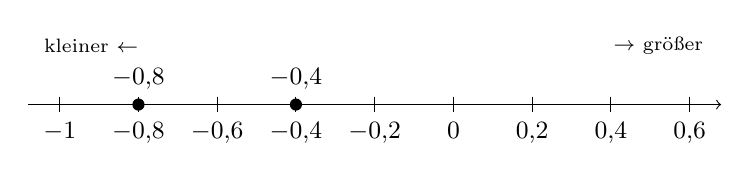
\begin{tikzpicture}[scale=1.0,font=\small]\draw[->] (-5.4,0) -- (3.4,0);\foreach \x/\l in {-5/-1,-4/-0{,}8,-3/-0{,}6,-2/-0{,}4,-1/-0{,}2,0/0,1/0{,}2,2/0{,}4,3/0{,}6}{\draw (\x,0.1) -- (\x,-0.1) node[below] {$\l$};}\fill (-4,0) circle (2.2pt) node[above=2pt] {$-0{,}8$};\fill (-2,0) circle (2.2pt) node[above=2pt] {$-0{,}4$};\node[font=\scriptsize] at (-4.6,0.75) {kleiner $\leftarrow$};\node[font=\scriptsize] at (2.6,0.75) {$\rightarrow$ größer};\end{tikzpicture}
\end{minipage}
\end{tcolorbox}
\medskip\noindent\textbf{Typische Fehler – so nicht}\par\smallskip
\noindent\nr{$\times$}Nach der Länge verglichen: $0{,}066$ ist nicht größer als $0{,}6$.\par
\noindent\nr{$\times$}Bei negativen Zahlen wie bei positiven verglichen: $-0{,}5 < -0{,}45$, nicht umgekehrt.\par
\noindent\nr{$\times$}Quadrat verdoppelt: $0{,}4^2 = 0{,}16$, nicht $0{,}8$.\par
\noindent\nr{$\times$}Prozent nur um eine Stelle verschoben: $7\,\% = 0{,}07$, nicht $0{,}7$.\par
\noindent\nr{$\times$}Wurzel als die Zahl selbst gelesen: $\sqrt{2} \approx 1{,}41$, nicht 2.\par
\clearpage\label{s:A}\noindent\colorbox{black!12}{\makebox[10mm]{\Large\bfseries\strut A}}\hspace{3mm}{\Large\bfseries Dezimalzahlen vergleichen}\par\smallskip
\noindent Hänge Nullen an, bis beide Zahlen gleich viele Stellen nach dem Komma haben – das ändert den Wert nicht. Dann vergleichst du Stelle für Stelle von links: Die erste Stelle, an der sie sich unterscheiden, entscheidet.\par\medskip
\noindent\textbf{Formel}\par\nopagebreak\noindent\hspace*{4mm}\begin{minipage}{\dimexpr\linewidth-4mm\relax}$0{,}7 = 0{,}70$ \qquad $0{,}70 > 0{,}65$, \ denn 7 Zehntel $>$ 6 Zehntel\end{minipage}\par\medskip
\noindent\textbf{Beispiel}\quad Setze $<$, $>$ oder $=$: \ $0{,}7$ \leerfeld $0{,}65$\par\smallskip
\noindent\par\noindent\hangindent6mm\hangafter1\makebox[6mm][l]{\textbf{1}}Eine Null anhängen ändert den Wert nicht: $0{,}7 = 0{,}70$.\newline $0{,}70$ und $0{,}65$\par\smallskip\par\noindent\hangindent6mm\hangafter1\makebox[6mm][l]{\textbf{2}}Von links vergleichen: Einer gleich, die Zehntel entscheiden.\newline 7 Zehntel $>$ 6 Zehntel, also $0{,}7 > 0{,}65$\par\smallskip\par\medskip
\noindent\textbf{Aufgaben}\hspace{1em}{\small\color{mbgrau}\karohinweis{A}{Rechne unten im Karo.}{Rechne auf einem extra Blatt.} Vergleiche jede Aufgabe gleich mit dem Lösungsheft.}\par\smallskip
\aufg{\nr{1.}\begin{minipage}[t]{\dimexpr\linewidth-7mm\relax}Wo entscheidet es sich? Nenne nur die Stelle, an der sich die zwei Zahlen zuerst unterscheiden (Einer, Zehntel, Hundertstel, Tausendstel). Noch kein Zeichen setzen.\par\smallskip
\grau{a)\ $3{,}47$ und $3{,}42$:\quad Einer gleich, Zehntel gleich, Hundertstel verschieden $\Rightarrow$ Hundertstel}\par{\small Lies von links: Einer 3 und 3, Zehntel 4 und 4, Hundertstel 7 und 2 – hier zuerst verschieden.}\par\medskip
\noindent\begin{minipage}[t]{0.48\linewidth}\raggedright
b)\ $0{,}81$ und $0{,}91$\linie{25mm}
\end{minipage}\hfill
\begin{minipage}[t]{0.48\linewidth}\raggedright
c)\ $12{,}305$ und $12{,}308$\linie{25mm}
\end{minipage}\par\smallskip
\noindent\begin{minipage}[t]{0.48\linewidth}\raggedright
d)\ $7{,}25$ und $6{,}25$\linie{25mm}
\end{minipage}\hfill
\begin{minipage}[t]{0.48\linewidth}\raggedright
e)\ $0{,}406$ und $0{,}46$\linie{25mm}
\end{minipage}\par\smallskip\end{minipage}}{}{}
\medskip
\aufg{\nr{2.}\begin{minipage}[t]{\dimexpr\linewidth-7mm\relax}Hänge Nullen an, bis beide Zahlen gleich viele Stellen nach dem Komma haben. Setze dann $<$, $>$ oder $=$.\par\smallskip
\noindent\begin{minipage}[t]{0.48\linewidth}\raggedright
a)\ $2{,}4$ \fbox{\phantom{$<$}} $2{,}38$\linie{25mm}
\end{minipage}\hfill
\begin{minipage}[t]{0.48\linewidth}\raggedright
b)\ $0{,}09$ \fbox{\phantom{$<$}} $0{,}1$\linie{25mm}
\end{minipage}\par\smallskip
\noindent\begin{minipage}[t]{0.48\linewidth}\raggedright
c)\ $5{,}05$ \fbox{\phantom{$<$}} $5{,}5$\linie{25mm}
\end{minipage}\hfill
\begin{minipage}[t]{0.48\linewidth}\raggedright
d)\ $1{,}250$ \fbox{\phantom{$<$}} $1{,}25$\linie{25mm}
\end{minipage}\par\smallskip\end{minipage}}{}{}
\medskip
\aufg{\hangindent7mm\hangafter1\nr{3.}Ordne von klein nach groß: $0{,}6$; \ $0{,}06$; \ $0{,}066$; \ $0{,}61$.}{}{{\scriptsize\color{mbgrau}Ziel\hspace{2mm}}}
\medskip
\par\vspace{3mm}\setlength{\kr}{\dimexpr\pagegoal-\pagetotal-10mm\relax}%
\ifdim\kr>12mm\karomerk{k}{A}\noindent{\scriptsize\color{mbgrau}Platz zum Rechnen}\par\nointerlineskip\vspace{1mm}\noindent
\begin{tikzpicture}\clip (0,0) rectangle ({\linewidth-0.5mm},\kr);\draw[black!16,line width=0.3pt,step=5mm] (0,0) grid (\linewidth,\kr);\end{tikzpicture}\fi\par
\clearpage\label{s:B}\noindent\colorbox{black!12}{\makebox[10mm]{\Large\bfseries\strut B}}\hspace{3mm}{\Large\bfseries Negative Zahlen vergleichen}\par\smallskip
\noindent Auf der Zahlengeraden ist links kleiner. Von zwei negativen Zahlen ist die kleiner, die weiter von 0 weg ist. Die Mitte findest du über den halben Abstand.\par\medskip
\noindent\textbf{Formel}\par\nopagebreak\noindent\hspace*{4mm}\begin{minipage}{\dimexpr\linewidth-4mm\relax}$-0{,}8 < -0{,}4 < 0 < 0{,}4$ \par\vspace{4pt} Mitte $=$ kleinere Zahl $+$ Abstand $: 2$\end{minipage}\par\medskip
\noindent\textbf{Beispiel}\quad Welche Zahl liegt auf der Zahlengeraden weiter links: $-0{,}8$ oder $-0{,}4$?\par\smallskip
\noindent\begin{minipage}[t]{0.6\linewidth}\vspace{0pt}\par\noindent\hangindent6mm\hangafter1\makebox[6mm][l]{\textbf{1}}Beide sind negativ. $-0{,}8$ ist weiter von 0 weg als $-0{,}4$, also weiter links.\newline $-0{,}8$ liegt links von $-0{,}4$, also $-0{,}8 < -0{,}4$\par\smallskip\end{minipage}\hfill
\begin{minipage}[t]{0.37\linewidth}\vspace{0pt}\centering 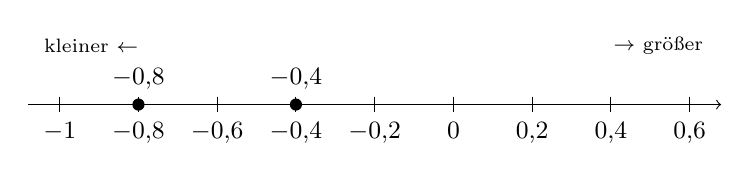
\begin{tikzpicture}[scale=1.0,font=\small]\draw[->] (-5.4,0) -- (3.4,0);\foreach \x/\l in {-5/-1,-4/-0{,}8,-3/-0{,}6,-2/-0{,}4,-1/-0{,}2,0/0,1/0{,}2,2/0{,}4,3/0{,}6}{\draw (\x,0.1) -- (\x,-0.1) node[below] {$\l$};}\fill (-4,0) circle (2.2pt) node[above=2pt] {$-0{,}8$};\fill (-2,0) circle (2.2pt) node[above=2pt] {$-0{,}4$};\node[font=\scriptsize] at (-4.6,0.75) {kleiner $\leftarrow$};\node[font=\scriptsize] at (2.6,0.75) {$\rightarrow$ größer};\end{tikzpicture}\end{minipage}\par\medskip
\noindent\textbf{Aufgaben}\hspace{1em}{\small\color{mbgrau}\karohinweis{B}{Rechne unten im Karo.}{Rechne auf einem extra Blatt.} Vergleiche jede Aufgabe gleich mit dem Lösungsheft.}\par\smallskip
\aufg{\nr{1.}\begin{minipage}[t]{\dimexpr\linewidth-7mm\relax}Welche Zahl liegt auf der Zahlengeraden weiter links? Schreib sie auf. Die liegt weiter links, ist die kleinere.\par\smallskip
\noindent\begin{minipage}[t]{0.48\linewidth}\raggedright
a)\ $-2$ und $1$\linie{25mm}
\end{minipage}\hfill
\begin{minipage}[t]{0.48\linewidth}\raggedright
b)\ $-0{,}5$ und $0{,}3$\linie{25mm}
\end{minipage}\par\smallskip
\noindent\begin{minipage}[t]{0.48\linewidth}\raggedright
c)\ $-3$ und $-1$\linie{25mm}
\end{minipage}\hfill
\begin{minipage}[t]{0.48\linewidth}\raggedright
d)\ $0$ und $-0{,}1$\linie{25mm}
\end{minipage}\par\smallskip\end{minipage}}{}{}
\medskip
\aufg{\nr{2.}\begin{minipage}[t]{\dimexpr\linewidth-7mm\relax}Setze $<$ oder $>$. Bei zwei negativen Zahlen: Die weiter von 0 weg ist, ist die kleinere.\par\smallskip
\grau{a)\ $-0{,}6$ \fbox{\phantom{$<$}} $-0{,}65$:\quad $0{,}60 < 0{,}65$: \ $-0{,}65$ ist weiter von 0 weg\quad$\Rightarrow$\quad $-0{,}6 > -0{,}65$}\par{\small Ohne Minus vergleichen (mit Null angehängt). Bei den negativen dreht sich das Zeichen um.}\par\medskip
\noindent\begin{minipage}[t]{0.48\linewidth}\raggedright
b)\ $-1{,}2$ \fbox{\phantom{$<$}} $-1{,}02$\linie{25mm}
\end{minipage}\hfill
\begin{minipage}[t]{0.48\linewidth}\raggedright
c)\ $-0{,}3$ \fbox{\phantom{$<$}} $0{,}1$\linie{25mm}
\end{minipage}\par\smallskip
\noindent\begin{minipage}[t]{0.48\linewidth}\raggedright
d)\ $-2{,}5$ \fbox{\phantom{$<$}} $-2{,}45$\linie{25mm}
\end{minipage}\hfill
\begin{minipage}[t]{0.48\linewidth}\raggedright
e)\ $-0{,}09$ \fbox{\phantom{$<$}} $-0{,}1$\linie{25mm}
\end{minipage}\par\smallskip\end{minipage}}{}{}
\medskip
\aufg{\nr{3.}\begin{minipage}[t]{\dimexpr\linewidth-7mm\relax}Welche Zahl liegt genau in der Mitte? Rechne den Abstand aus, halbiere ihn und geh von der kleineren Zahl so weit nach rechts.\par\smallskip
\grau{a)\ $-0{,}8$ und $-0{,}5$:\quad Abstand $0{,}3$, Hälfte $0{,}15$\quad$\Rightarrow$\quad $-0{,}8 + 0{,}15 = -0{,}65$}\par{\small Von $-0{,}8$ bis $-0{,}5$ sind es 3 Zehntel. Von der kleineren Zahl den halben Abstand nach rechts.}\par\medskip
\noindent\begin{minipage}[t]{0.48\linewidth}\raggedright
b)\ $-0{,}4$ und $-0{,}2$
\end{minipage}\hfill
\begin{minipage}[t]{0.48\linewidth}\raggedright
c)\ $-1$ und $-0{,}6$
\end{minipage}\par\smallskip
\noindent\begin{minipage}[t]{0.48\linewidth}\raggedright
d)\ $-0{,}3$ und $0{,}1$
\end{minipage}\par\smallskip
\par{\small Probe: Die Mitte liegt zwischen den beiden Zahlen und ist von beiden gleich weit weg.}\end{minipage}}{}{}
\medskip
\aufg{\hangindent7mm\hangafter1\nr{4.}Temperaturen am Morgen: Oslo $-3{,}5$\,°C, \ Riga $-3{,}05$\,°C, \ Wien $0{,}5$\,°C, \ Prag $-0{,}8$\,°C, \ Kiew $-4$\,°C. Ordne die Städte von kalt nach warm. Wo war es am kältesten?}{}{{\scriptsize\color{mbgrau}Ziel\hspace{2mm}}}
\medskip
\par\vspace{3mm}\setlength{\kr}{\dimexpr\pagegoal-\pagetotal-10mm\relax}%
\ifdim\kr>12mm\karomerk{k}{B}\noindent{\scriptsize\color{mbgrau}Platz zum Rechnen}\par\nointerlineskip\vspace{1mm}\noindent
\begin{tikzpicture}\clip (0,0) rectangle ({\linewidth-0.5mm},\kr);\draw[black!16,line width=0.3pt,step=5mm] (0,0) grid (\linewidth,\kr);\end{tikzpicture}\fi\par
\clearpage\label{s:C}\noindent\colorbox{black!12}{\makebox[10mm]{\Large\bfseries\strut C}}\hspace{3mm}{\Large\bfseries Bruch und Prozent: erst umwandeln}\par\smallskip
\noindent Bring alle Zahlen in dieselbe Form: Dezimalzahl. Beim Bruch erweiterst du den Nenner auf 10, 100 oder 1000; Prozent heißt Hundertstel.\par\medskip
\noindent\textbf{Formel}\par\nopagebreak\noindent\hspace*{4mm}\begin{minipage}{\dimexpr\linewidth-4mm\relax}$\dfrac{3}{4} = \dfrac{75}{100} = 0{,}75$ \qquad $7\,\% = \dfrac{7}{100} = 0{,}07$\end{minipage}\par\medskip
\noindent\textbf{Beispiel}\quad Schreib $\frac{3}{5}$ als Dezimalzahl.\par\smallskip
\noindent\par\noindent\hangindent6mm\hangafter1\makebox[6mm][l]{\textbf{1}}Mit 2 erweitern: Nenner 10, also Zehntel.\newline $\frac{3}{5} = \frac{6}{10} = 0{,}6$\par\smallskip\par\medskip
\noindent\textbf{Aufgaben}\hspace{1em}{\small\color{mbgrau}\karohinweis{C}{Rechne unten im Karo.}{Rechne auf einem extra Blatt.} Vergleiche jede Aufgabe gleich mit dem Lösungsheft.}\par\smallskip
\aufg{\nr{1.}\begin{minipage}[t]{\dimexpr\linewidth-7mm\relax}Schreib den Bruch als Dezimalzahl: Erweitere den Nenner auf 10, 100 oder 1000.\par\smallskip
\noindent\begin{minipage}[t]{0.48\linewidth}\raggedright
a)\ $\dfrac{3}{4}$
\end{minipage}\hfill
\begin{minipage}[t]{0.48\linewidth}\raggedright
b)\ $\dfrac{7}{20}$
\end{minipage}\par\smallskip
\noindent\begin{minipage}[t]{0.48\linewidth}\raggedright
c)\ $\dfrac{1}{8}$
\end{minipage}\hfill
\begin{minipage}[t]{0.48\linewidth}\raggedright
d)\ $\dfrac{9}{25}$
\end{minipage}\par\smallskip\end{minipage}}{}{}
\medskip
\aufg{\nr{2.}\begin{minipage}[t]{\dimexpr\linewidth-7mm\relax}Schreib als Dezimalzahl. Prozent heißt Hundertstel: Komma zwei Stellen nach links.\par\smallskip
\grau{a)\ $7\,\%$:\quad $7\,\% = \frac{7}{100} = 0{,}07$}\par{\small 7 Hundertstel: die 7 steht an der zweiten Stelle nach dem Komma.}\par\medskip
\noindent\begin{minipage}[t]{0.48\linewidth}\raggedright
b)\ $45\,\%$
\end{minipage}\hfill
\begin{minipage}[t]{0.48\linewidth}\raggedright
c)\ $4{,}5\,\%$
\end{minipage}\par\smallskip
\noindent\begin{minipage}[t]{0.48\linewidth}\raggedright
d)\ $120\,\%$
\end{minipage}\hfill
\begin{minipage}[t]{0.48\linewidth}\raggedright
e)\ $0{,}5\,\%$
\end{minipage}\par\smallskip\end{minipage}}{}{}
\medskip
\aufg{\nr{3.}\begin{minipage}[t]{\dimexpr\linewidth-7mm\relax}Wandle erst in Dezimalzahlen um, dann vergleiche. Setze $<$, $>$ oder $=$.\par\smallskip
\grau{a)\ $\dfrac{3}{4}$ \fbox{\phantom{$<$}} $0{,}8$:\quad $\frac{3}{4} = 0{,}75$\quad$\Rightarrow$\quad $0{,}75 < 0{,}80$, also $\frac{3}{4} < 0{,}8$}\par{\small Den Bruch umwandeln. Dann wie in A: Nullen anhängen, von links vergleichen.}\par\medskip
\noindent\begin{minipage}[t]{0.48\linewidth}\raggedright
b)\ $6\,\%$ \fbox{\phantom{$<$}} $0{,}6$
\end{minipage}\hfill
\begin{minipage}[t]{0.48\linewidth}\raggedright
c)\ $0{,}35$ \fbox{\phantom{$<$}} $\dfrac{7}{20}$
\end{minipage}\par\smallskip
\noindent\begin{minipage}[t]{0.48\linewidth}\raggedright
d)\ $\dfrac{2}{5}$ \fbox{\phantom{$<$}} $45\,\%$
\end{minipage}\hfill
\begin{minipage}[t]{0.48\linewidth}\raggedright
e)\ $\dfrac{1}{8}$ \fbox{\phantom{$<$}} $0{,}13$
\end{minipage}\par\smallskip\end{minipage}}{}{{\scriptsize\color{mbgrau}Ziel\hspace{2mm}}}
\medskip
\par\vspace{3mm}\setlength{\kr}{\dimexpr\pagegoal-\pagetotal-10mm\relax}%
\ifdim\kr>12mm\karomerk{k}{C}\noindent{\scriptsize\color{mbgrau}Platz zum Rechnen}\par\nointerlineskip\vspace{1mm}\noindent
\begin{tikzpicture}\clip (0,0) rectangle ({\linewidth-0.5mm},\kr);\draw[black!16,line width=0.3pt,step=5mm] (0,0) grid (\linewidth,\kr);\end{tikzpicture}\fi\par
\clearpage\label{s:D}\noindent\colorbox{black!12}{\makebox[10mm]{\Large\bfseries\strut D}}\hspace{3mm}{\Large\bfseries Quadrat und Wurzel}\par\smallskip
\noindent Das Quadrat ist die Zahl mal sich selbst, nicht mal 2. Die Wurzel fragt rückwärts: Welche Zahl mal sich selbst gibt das? Geht sie nicht auf, schließt du sie zwischen zwei Zehnteln ein.\par\medskip
\noindent\textbf{Formel}\par\nopagebreak\noindent\hspace*{4mm}\begin{minipage}{\dimexpr\linewidth-4mm\relax}$0{,}4^2 = 0{,}4 \cdot 0{,}4 = 0{,}16$ \qquad $\sqrt{0{,}16} = 0{,}4$ \par\vspace{4pt} $1{,}4^2 = 1{,}96 < 2 < 2{,}25 = 1{,}5^2$, \ also $1{,}4 < \sqrt{2} < 1{,}5$\end{minipage}\par\medskip
\noindent\textbf{Beispiel}\quad Rechne aus: $0{,}4^2$\par\smallskip
\noindent\par\noindent\hangindent6mm\hangafter1\makebox[6mm][l]{\textbf{1}}$4 \cdot 4 = 16$; eine Stelle mal eine Stelle gibt zwei Stellen nach dem Komma.\newline $0{,}4^2 = 0{,}4 \cdot 0{,}4 = 0{,}16$\par\smallskip\par\medskip
\noindent\textbf{Aufgaben}\hspace{1em}{\small\color{mbgrau}\karohinweis{D}{Rechne unten im Karo.}{Rechne auf einem extra Blatt.} Vergleiche jede Aufgabe gleich mit dem Lösungsheft.}\par\smallskip
\aufg{\nr{1.}\begin{minipage}[t]{\dimexpr\linewidth-7mm\relax}Rechne das Quadrat aus: die Zahl mal sich selbst – nicht mal 2.\par\smallskip
\noindent\begin{minipage}[t]{0.48\linewidth}\raggedright
a)\ $0{,}2^2$
\end{minipage}\hfill
\begin{minipage}[t]{0.48\linewidth}\raggedright
b)\ $0{,}5^2$
\end{minipage}\par\smallskip
\noindent\begin{minipage}[t]{0.48\linewidth}\raggedright
c)\ $1{,}1^2$
\end{minipage}\hfill
\begin{minipage}[t]{0.48\linewidth}\raggedright
d)\ $0{,}1^2$
\end{minipage}\par\smallskip\end{minipage}}{}{}
\medskip
\aufg{\nr{2.}\begin{minipage}[t]{\dimexpr\linewidth-7mm\relax}Zieh die Wurzel: Welche Zahl mal sich selbst gibt die Zahl unter der Wurzel? Prüfe mit dem Quadrat.\par\smallskip
\grau{a)\ $\sqrt{0{,}25}$:\quad $0{,}5 \cdot 0{,}5 = 0{,}25$, also $\sqrt{0{,}25} = 0{,}5$}\par{\small $5 \cdot 5 = 25$; zwei Stellen unter der Wurzel, eine Stelle im Ergebnis.}\par\medskip
\noindent\begin{minipage}[t]{0.48\linewidth}\raggedright
b)\ $\sqrt{0{,}09}$
\end{minipage}\hfill
\begin{minipage}[t]{0.48\linewidth}\raggedright
c)\ $\sqrt{1{,}44}$
\end{minipage}\par\smallskip
\noindent\begin{minipage}[t]{0.48\linewidth}\raggedright
d)\ $\sqrt{0{,}04}$
\end{minipage}\hfill
\begin{minipage}[t]{0.48\linewidth}\raggedright
e)\ $\sqrt{0{,}49}$
\end{minipage}\par\smallskip\end{minipage}}{}{}
\medskip
\aufg{\nr{3.}\begin{minipage}[t]{\dimexpr\linewidth-7mm\relax}Die Wurzel geht nicht auf. Zwischen welchen zwei Zehnteln liegt sie? Probiere Quadrate, bis die Zahl dazwischen liegt.\par\smallskip
\grau{a)\ $\sqrt{2}$:\quad $1{,}4^2 = 1{,}96$, \ $1{,}5^2 = 2{,}25$\quad$\Rightarrow$\quad $1{,}4 < \sqrt{2} < 1{,}5$}\par{\small $1{,}4 \cdot 1{,}4 = 1{,}96$ ist knapp unter 2, $1{,}5 \cdot 1{,}5 = 2{,}25$ schon darüber. Also liegt die Wurzel dazwischen, etwa bei $1{,}41$.}\par\medskip
\noindent\begin{minipage}[t]{0.48\linewidth}\raggedright
b)\ $\sqrt{3}$
\end{minipage}\hfill
\begin{minipage}[t]{0.48\linewidth}\raggedright
c)\ $\sqrt{5}$
\end{minipage}\par\smallskip
\noindent\begin{minipage}[t]{0.48\linewidth}\raggedright
d)\ $\sqrt{0{,}5}$
\end{minipage}\par\smallskip\end{minipage}}{}{{\scriptsize\color{mbgrau}Ziel\hspace{2mm}}}
\medskip
\par\vspace{3mm}\setlength{\kr}{\dimexpr\pagegoal-\pagetotal-10mm\relax}%
\ifdim\kr>12mm\karomerk{k}{D}\noindent{\scriptsize\color{mbgrau}Platz zum Rechnen}\par\nointerlineskip\vspace{1mm}\noindent
\begin{tikzpicture}\clip (0,0) rectangle ({\linewidth-0.5mm},\kr);\draw[black!16,line width=0.3pt,step=5mm] (0,0) grid (\linewidth,\kr);\end{tikzpicture}\fi\par
\clearpage\label{s:E}\noindent\colorbox{black!12}{\makebox[10mm]{\Large\bfseries\strut E}}\hspace{3mm}{\Large\bfseries Alles gemischt: vergleichen und entscheiden}\par\smallskip
\noindent Schreib jede Zahl als Dezimalzahl daneben, dann vergleichst du wie in A und B. Negative Zahlen kommen nach links. In Sachaufgaben: erst die Zahlen finden, am Ende die Frage beantworten.\par\medskip
\noindent\textbf{Formel}\par\nopagebreak\noindent\hspace*{4mm}\begin{minipage}{\dimexpr\linewidth-4mm\relax}Bruch, Prozent, Quadrat, Wurzel \ $\to$ \ Dezimalzahl \ $\to$ \ Nullen anhängen \ $\to$ \ von links vergleichen\end{minipage}\par\medskip
\noindent\textbf{Beispiel}\quad Welcher Wert ist der kleinste? Kreuze an. \kreuz{$0{,}7$} \kreuz{$0{,}1^2$} \kreuz{$3\,\%$} \kreuz{$0{,}025$}\par\smallskip
\noindent\par\noindent\hangindent6mm\hangafter1\makebox[6mm][l]{\textbf{1}}Alles in Dezimalzahlen mit drei Stellen.\newline $0{,}7 = 0{,}700$; \ $0{,}1^2 = 0{,}010$; \ $3\,\% = 0{,}030$; \ $0{,}025$\par\smallskip\par\noindent\hangindent6mm\hangafter1\makebox[6mm][l]{\textbf{2}}Von links vergleichen.\newline Zehntel: nur $0{,}700$ hat welche. Hundertstel: $0{,}010$ hat 1, die anderen 2 und 3.\par\smallskip\par\noindent\hangindent6mm\hangafter1\makebox[6mm][l]{\textbf{3}}Der kleinste ist $0{,}1^2 = 0{,}01$.\par\smallskip\par\medskip
\noindent\textbf{Aufgaben}\hspace{1em}{\small\color{mbgrau}\karohinweis{E}{Rechne unten im Karo.}{Rechne auf einem extra Blatt.} Vergleiche jede Aufgabe gleich mit dem Lösungsheft.}\par\smallskip
\aufg{\hangindent7mm\hangafter1\nr{1.}Welcher Wert ist der kleinste? Kreuze an.\par\smallskip\leftskip7mm \kreuz{$0{,}9$}\ \kreuz{$0{,}3^2$}\par\kreuz{$8\,\%$}\ \kreuz{$0{,}085$}}{}{}
\medskip
\aufg{\hangindent7mm\hangafter1\nr{2.}Ordne von klein nach groß: \ $0{,}3$; \ $-\frac{3}{4}$; \ $\sqrt{0{,}16}$; \ $-0{,}7$.}{}{}
\medskip
\aufg{\hangindent7mm\hangafter1\nr{3.}Nur eine Aussage ist wahr. Kreuze sie an.\par\medskip\noindent\hspace*{7mm}\mbox{$\square$\ $\sqrt{2} > \dfrac{3}{2}$}\hspace{10mm}\mbox{$\square$\ $0{,}3^2 > 0{,}3$}\hspace{10mm}\mbox{$\square$\ $-0{,}5 < -\dfrac{3}{5}$}\hspace{10mm}\mbox{$\square$\ $\dfrac{5}{8} > 0{,}6$}\rule[-3mm]{0pt}{8mm}\par\smallskip }{}{}
\medskip
\aufg{\hangindent7mm\hangafter1\nr{4.}Drei Läden haben dieselbe Jacke. Laden A: „Ein Viertel billiger!“ \ Laden B: „22\,\% Rabatt“ \ Laden C: „Jeden fünften Euro schenken wir dir!“ \ Wo ist der Rabatt am größten? Um wie viele Prozentpunkte ist er größer als beim zweitbesten Laden?}{}{}
\medskip
\aufg{\hangindent7mm\hangafter1\nr{5.}Mia taucht in $4{,}8$\,m Tiefe, ihr Bruder in $2{,}4$\,m Tiefe. Genau in der Mitte zwischen beiden schwimmt ein Fisch. Ein Foto gelingt nur tiefer als $3{,}5$\,m. Kann Mia den Fisch fotografieren?}{}{{\scriptsize\color{mbgrau}Ziel\hspace{2mm}}}
\medskip
\par\vspace{3mm}\setlength{\kr}{\dimexpr\pagegoal-\pagetotal-10mm\relax}%
\ifdim\kr>12mm\karomerk{k}{E}\noindent{\scriptsize\color{mbgrau}Platz zum Rechnen}\par\nointerlineskip\vspace{1mm}\noindent
\begin{tikzpicture}\clip (0,0) rectangle ({\linewidth-0.5mm},\kr);\draw[black!16,line width=0.3pt,step=5mm] (0,0) grid (\linewidth,\kr);\end{tikzpicture}\fi\par
\end{document}
